\documentclass[12pt]{article}
\usepackage{graphicx}
\usepackage{hyperref}
\title{Testing Policy}
\author{Binary Ninjaz}
\date{}

\hypersetup{
	colorlinks=true,
	linkcolor=black,
	filecolor=magenta,
	urlcolor=cyan,
}

% define the title
\author{Binary Ninjaz}
\title{Harvest}
\begin{document}
\begin{titlepage}

	\begin{center}
		% Upper part of the page
		\textsc{\LARGE Binary Ninjaz}\\[0.3cm]
		% Title
		\rule{\linewidth}{0.5mm} \\[0.5cm]
		{ \huge \bfseries Harvest \\
		  \vspace{0.3cm}\large \bfseries User Manual}\\[0.5cm]
		\rule{\linewidth}{0.5mm} \\[1cm]


		\begin{minipage}{0.4\textwidth}
			\begin{flushleft} \large
				\emph{} \\
				Letanyan {Arumugam}
			\end{flushleft}
		\end{minipage}
		\begin{minipage}{0.4\textwidth}
			\begin{flushright} \large
				\emph{} \\
				14228123
			\end{flushright}
		\end{minipage}

		\begin{minipage}{0.4\textwidth}
			\begin{flushleft} \large
            	\emph{} \\
				Sizo {Duma}
			\end{flushleft}
		\end{minipage}
		\begin{minipage}{0.4\textwidth}
			\begin{flushright} \large
				\emph{} \\
				15245579
			\end{flushright}
		\end{minipage}

		\begin{minipage}{0.4\textwidth}
			\begin{flushleft} \large
				\emph{} \\
				Teboho {Mokoena}
			\end{flushleft}
		\end{minipage}
		\begin{minipage}{0.4\textwidth}
			\begin{flushright} \large
				\emph{} \\
				14415888
			\end{flushright}
		\end{minipage}

		\begin{minipage}{0.4\textwidth}
			\begin{flushleft} \large
				\emph{} \\
				John {Ojo}
			\end{flushleft}
		\end{minipage}
		\begin{minipage}{0.4\textwidth}
			\begin{flushright} \large
				\emph{} \\
				15096794
			\end{flushright}
		\end{minipage}

        \begin{minipage}{0.4\textwidth}
			\begin{flushleft} \large
				\emph{} \\
				Kevin {Reid}
			\end{flushleft}
		\end{minipage}
		\begin{minipage}{0.4\textwidth}
			\begin{flushright} \large
				\emph{} \\
				15008739
			\end{flushright}
		\end{minipage}
        
        \begin{minipage}{0.4\textwidth}
			\begin{flushleft} \large
				\emph{} \\
				Shaun {Yates}
			\end{flushleft}
		\end{minipage}
		\begin{minipage}{0.4\textwidth}
			\begin{flushright} \large
				\emph{} \\
				16007493
			\end{flushright}
		\end{minipage}

		\vspace{1cm}
		\rule{\linewidth}{0.5mm} \\[1cm]
		\textsc{\Large Stakeholders}\\[1cm]

		\begin{minipage}{0.4\textwidth}
			\begin{flushleft} \large
				\emph{} \\
				SAMAC:
			\end{flushleft}
		\end{minipage}
		\begin{minipage}{0.4\textwidth}
			\begin{flushright} \large
				\emph{} \\
				Barry Christie
			\end{flushright}
		\end{minipage}


	\end{center}
\end{titlepage}

\newpage
\pagenumbering{Roman}
\tableofcontents
\newpage
\listoffigures

\newpage
\pagenumbering{arabic}
  
%\section{Introduction}
%Automated testing is vital in ensuring the number of defects in a program is as limited as possible. While having automated testing does not guarantee an absence of defects in a program it can greatly reduce that number; furthermore it serves to continually test and verify the function of modules that may be changed or affected upon by other changes.\\
%\indent While Binary Ninjaz intends to have as comprehensive test suite, they will not accept that wholly passing test cases means that a program is without flaw.\\
%\indent This document details the testing policies that are used by Binary Ninjaz in order to guide development and ensure a quality product; the specific testing methods used, and their impact of their effects on the general development process is described.

\section{Testing Process}
In this section, the testing process, based on IEEE-829, will illustrated. This process will fulfil the requirements stated in this document.\\
\indent Three phases within the testing process can be identified, namely:
\begin{enumerate}
	\item Test specification,
	\item Test implementation,
	\item Test reporting.
\end{enumerate}
Each phase is now elaborated.
\subsubsection{Test Specification}
The test specification can be subdivided into 2 parts. On the one hand, there is \textit{planning and verification}, on the other there is \textit{Analysis, design, and implementation}.\\
\indent \textit{Planning and verification} may consist of the following activities:
\begin{itemize}
 \item Specifying the scope and the risks, and defining the objectives of the tests;
\item Determining the strategy;
\item Taking decisions with regard to what must be tested, what roles apply, how the test activities will take place and how the outcomes of the tests will be implemented;
\item Planning of the test design activities;
\item Planning of implementation and evaluation.
\end{itemize}
During the \textit{analysis, design, and implementation} phase, the test objectives will be transformed into specific test conditions and test cases. This may involve the following activities:
\begin{itemize}
 \item A review of the test base (such as requirements, architecture, design, and interfaces);
\item Evaluation of the testability of the test base and the test objects;
\item Identification and prioritisation of the test conditions;
\item Designing of the test cases;
\item Identifying the necessary test data in order to support the test cases;
\item Designing the test environment and identifying the infrastructure and tools.
\end{itemize}
\subsubsection{Implementation of Tests}
The implementation of tests forms the phase in which the test procedures and scripts are implemented and the results of these (including incidents) are logged. This may involve the following activities:
\begin{itemize}
 \item Implementation of the tests, manually or by means of a tool;
\item Logging the results of the implementation;
\item Comparing the results with the result that had been predicted;
\item Reporting any setbacks in the form of incidents and analysing these in order to identify the cause;
\item Repeating the tests as a result of the incidents identified.
\end{itemize}
\subsubsection{Test Reporting}
Test Reporting forms the phase in which the implementation of the tests is compared with the objectives. This may involve the following tasks:
\begin{itemize}
 \item Checking of the test logs and the list of defects and comparing these to the exit criteria specified in the test plan;
\item Investigating whether additional tests are required;
\item Writing a summary report.
\end{itemize}
\subsection{Testing Frequency}
Since tests are used to validate the continued performance of a module---or the system as a whole---tests should be run after each module is finished being modified or created.

  \section{Testing Tools}
  There are many types of tests that can be run, in the case of \textbf{Harvest}, Unit and UI tests are run.
  \subsection{Android}
  \subsubsection{JUnit}
JUnit is a unit testing framework for the Java Environment, and as such is used for testing the Android---programmed in Java---implementation of \textbf{Harvest}. Android development is carried out using the Android Studio IDE, which facilitates easy use and set up of the JUnit framework. Android Studio also recommends the use of JUnit. For the reasons given, JUnit was selected to run unit tests on Android.\\
\indent Android unit tests can be found \href{https://github.com/BinaryNinjaz/COS301-Capstone/tree/master/Source/Android/Harvest/app/src/test/java/za/org/samac/harvest}{here}.

 \subsubsection{Espresso}
 Espresso, like JUnit, is integrated into, and recommended by, Android Studio, and therefore is used to facilitate UI testing on Android.\\
 \indent Android UI tests can be found \href{https://github.com/BinaryNinjaz/COS301-Capstone/tree/master/Source/Android/Harvest/app/src/androidTest/java/za/org/samac/harvest}{here}.
  
 \subsubsection{Execution}
   \begin{figure}
  	\includegraphics[width=\textwidth]{images/Android-JUnit-tests.png}
	\caption{Android Studio Test Example}
	\label{fig:android-test}
  \end{figure}
 Both UI and Unit tests are executed in the same manner for Android, the primary difference being that a UI test will need to run on a connected device or virtual machine.\\
\indent In order to run a unit or UI test for Android, one must open the file containing the desired test(s) using Android Studio as in figure \ref{fig:android-test}. Once there, one can right click on the green `test' button in the margin, then they can select to run the tests, the results of which will be seen at the bottom of the IDE.

\subsection{iOS}
\subsubsection{XCTest}
XCTest integrates seamlessly into Xcode's (the iOS IDE) testing workflow, and for that reason is used to facilitate all testing on iOS. XCTest is used for both UI and unit testing on iOS.\\
\indent iOS unit tests can be found \href{https://github.com/BinaryNinjaz/COS301-Capstone/tree/master/Source/iOS/Harvest/HarvestTests}{here}, and UI tests can be found \href{https://github.com/BinaryNinjaz/COS301-Capstone/tree/master/Source/iOS/Harvest/HarvestUITests}{here}.
\subsubsection{Execution}
To begin tests in Xcode, click on the play button in the top right, on the line that is highlighted in blue; as seen in figure \ref{fig:is}. This will run the tests. The results will look like figure \ref{fig:ie}.
  \begin{figure}
  	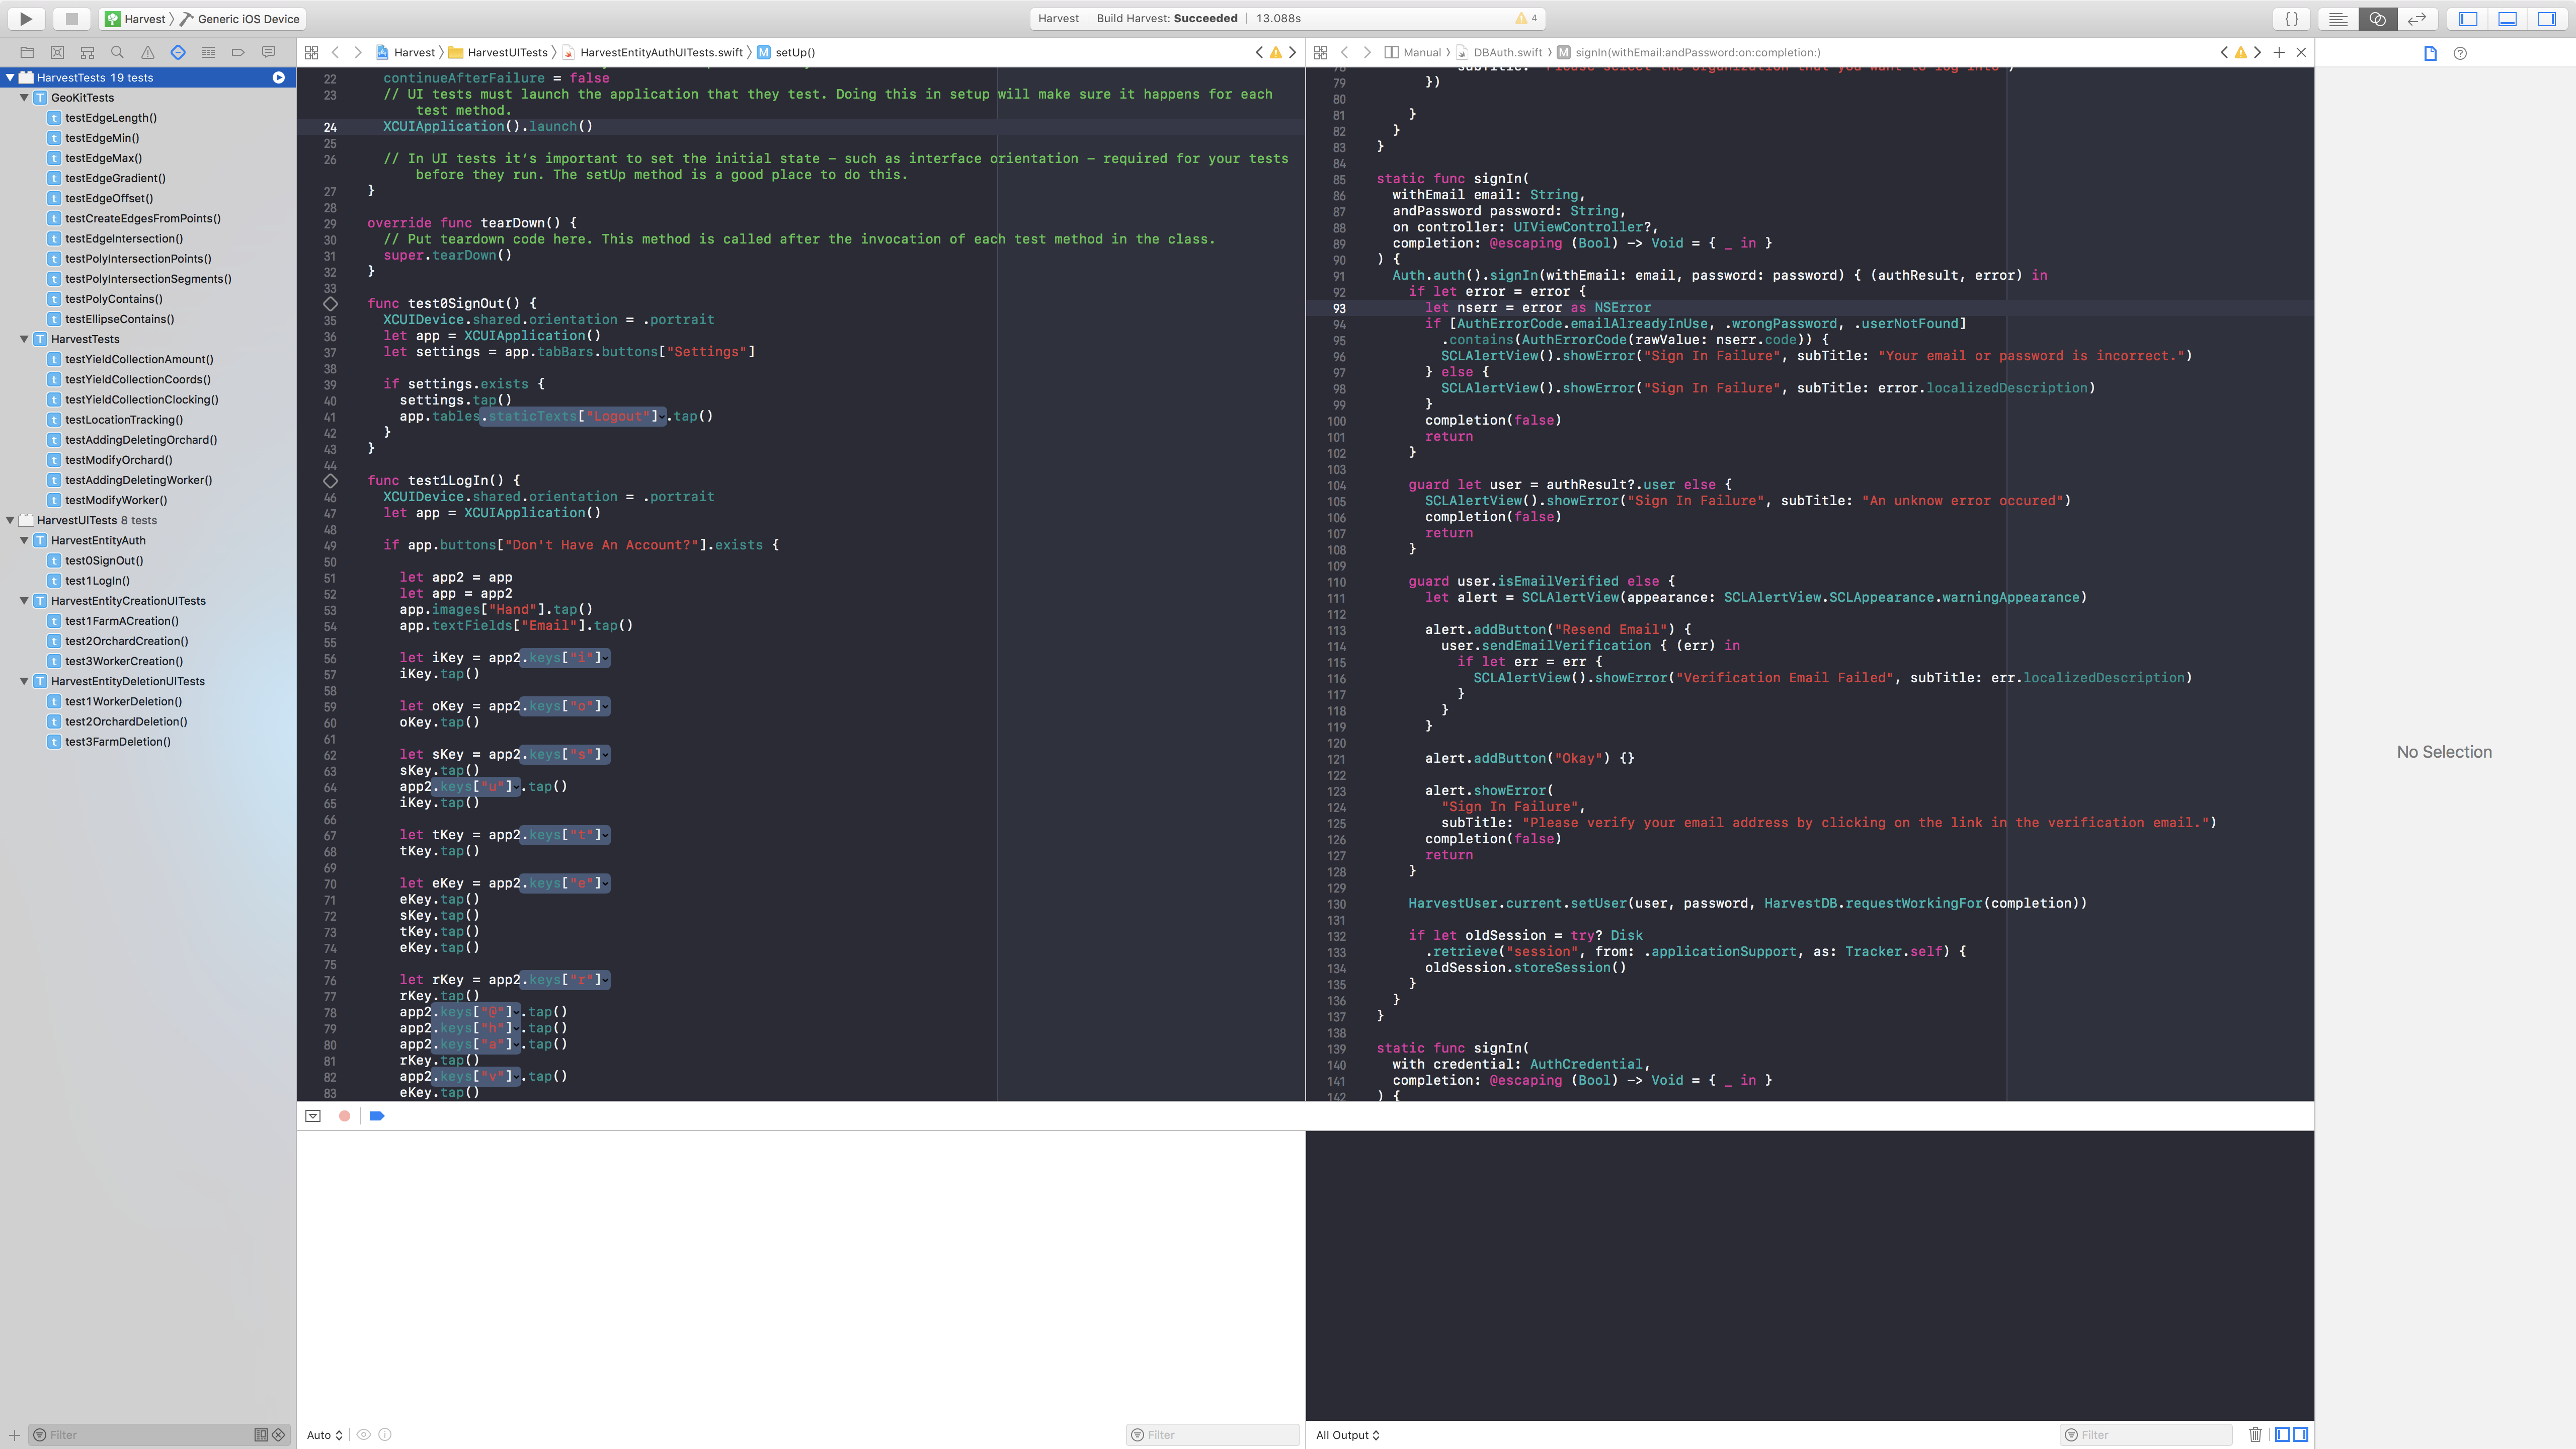
\includegraphics[width=\textwidth]{images/iOS-test.png}
	\caption{iOS Xcode Test Start}
	\label{fig:is}
  \end{figure}

\subsection{Web}
\subsubsection{QUnit}
QUnit is used for unit testing javascript functions. It was chosen since it displays its results in a convenient way---by including them in the web page, and it's very simple to use.\\
\indent QUnit tests can be found \href{https://github.com/BinaryNinjaz/COS301-Capstone/tree/master/Source/Web/app}{here}.
\subsubsection{Execution}
\begin{figure*}[ht!]
            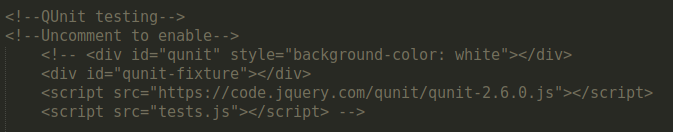
\includegraphics[width=.5\textwidth]{images/q1.png}
            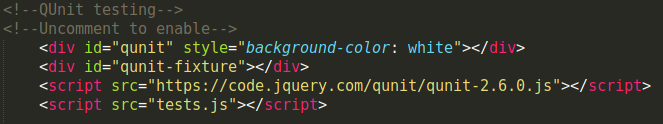
\includegraphics[width=.5\textwidth]{images/q2.png}
            \caption{Before Enabling Tests}
            \label{fig:q1}
            \caption{After Enabling Tests}
            \label{fig:q2}
        \end{figure*}
\paragraph{QUnit} To execute QUnit tests, go into the html file that uses the functions to be tested. At the bottom, find a segment that mentions \texttt{QUnit Testing}, such as in figure \ref{fig:q1}; then simply uncomment the code, as in figure \ref{fig:q2}, and refresh the page. The results are now displayed, such as in figure \ref{fig:qr}.

\begin{figure}
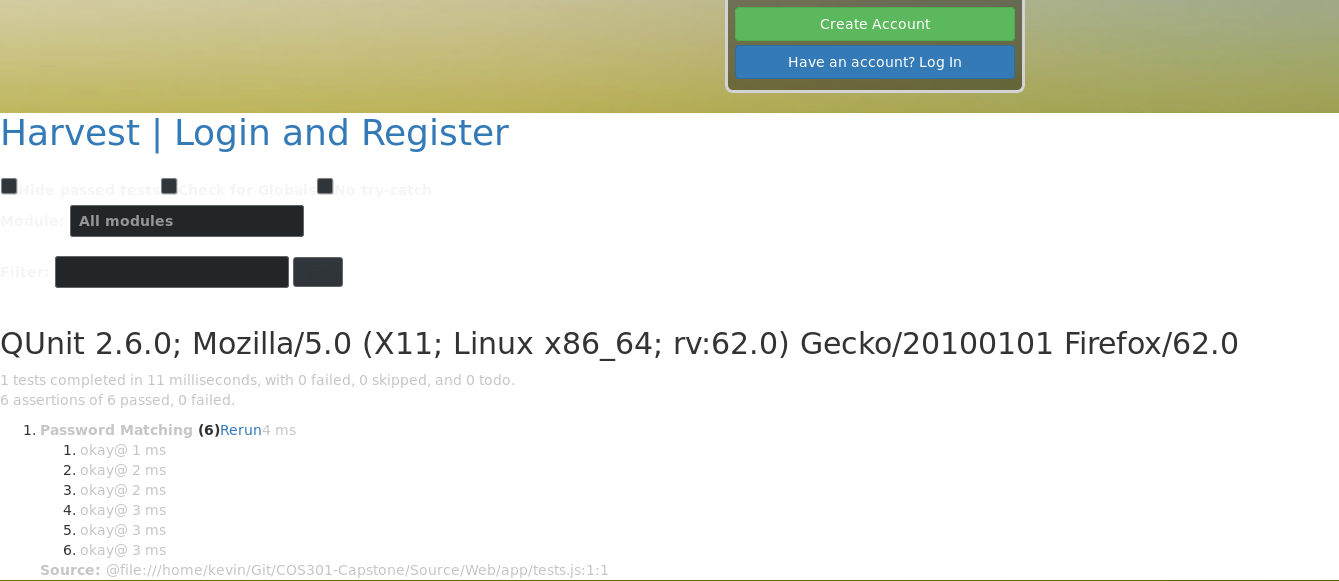
\includegraphics[width=\textwidth]{images/qr.png}
\caption{Results of QUnit test}
\label{fig:qr}
\end{figure}

\section{Test Cases}
TODO when requirements done.

\section{History}
\subsection{Android}
\begin{figure*}[ht!]
            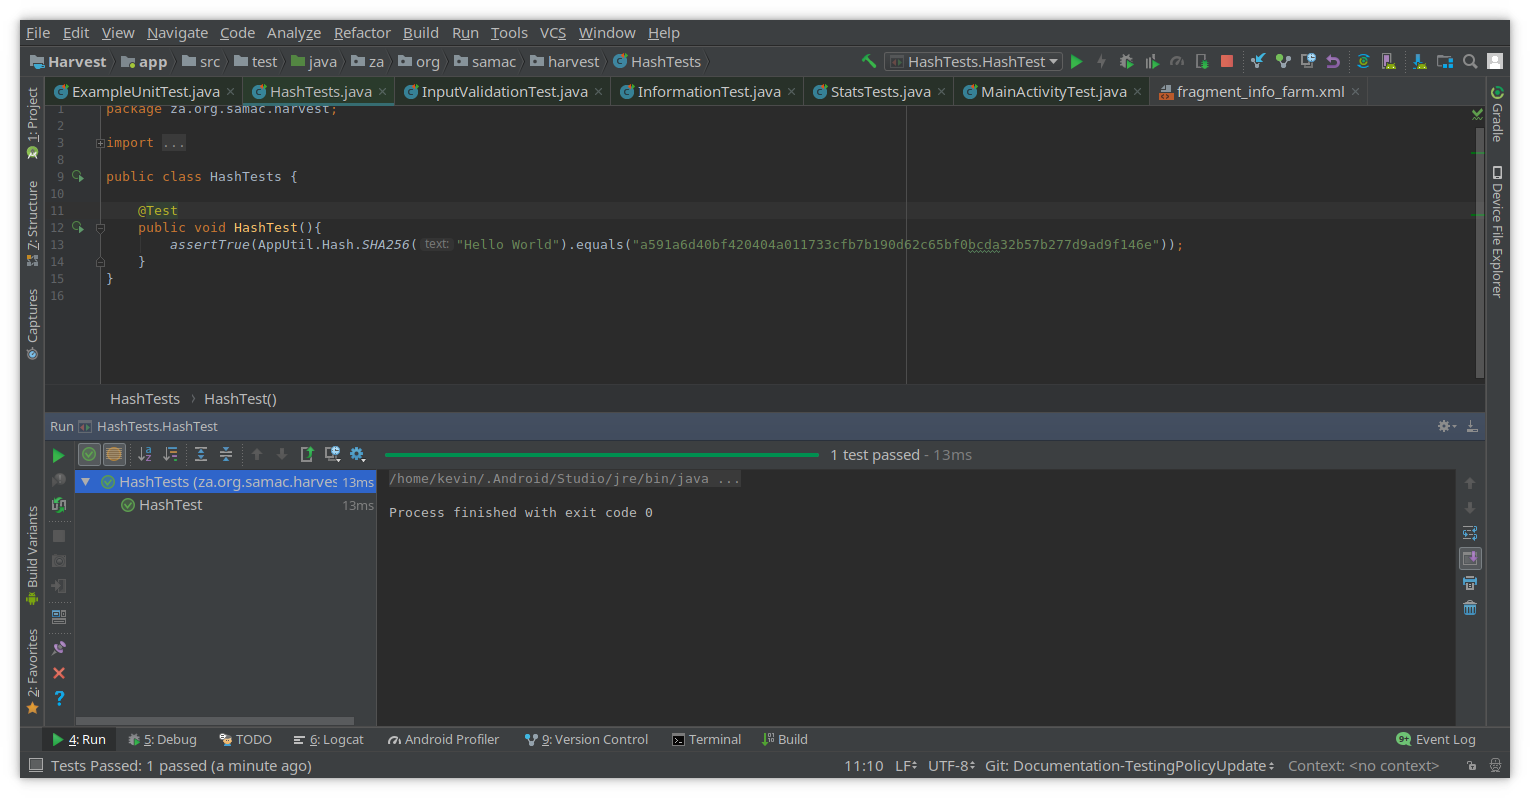
\includegraphics[width=.3\textwidth]{images/hash.png}
            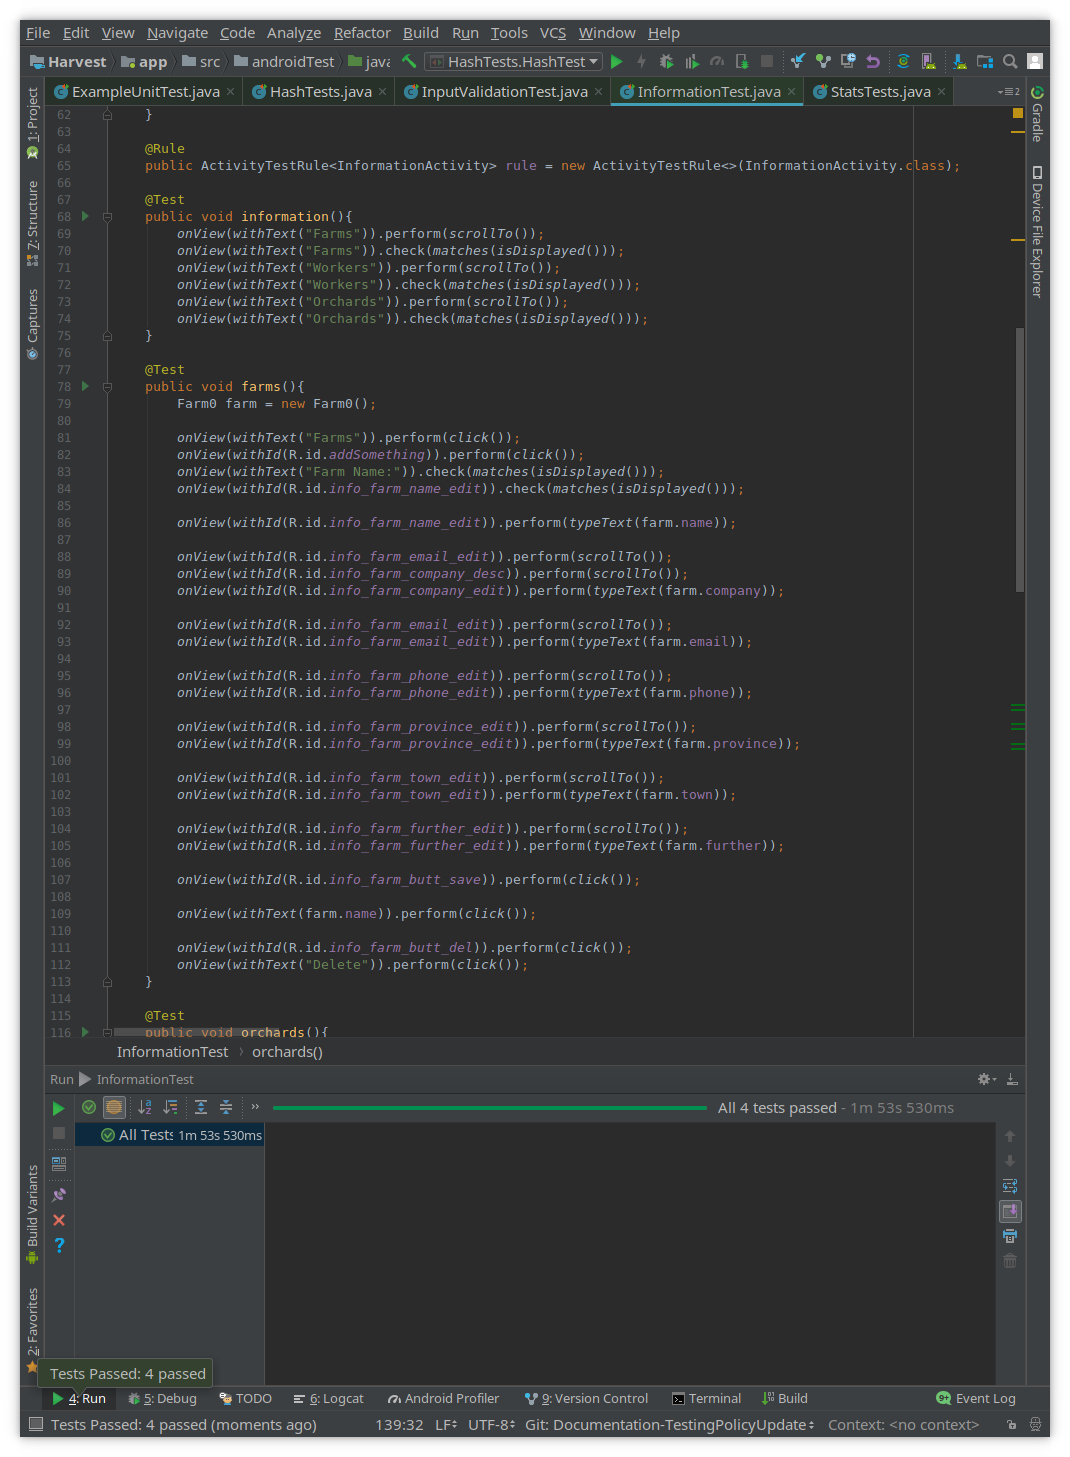
\includegraphics[width=.3\textwidth]{images/info.png}
            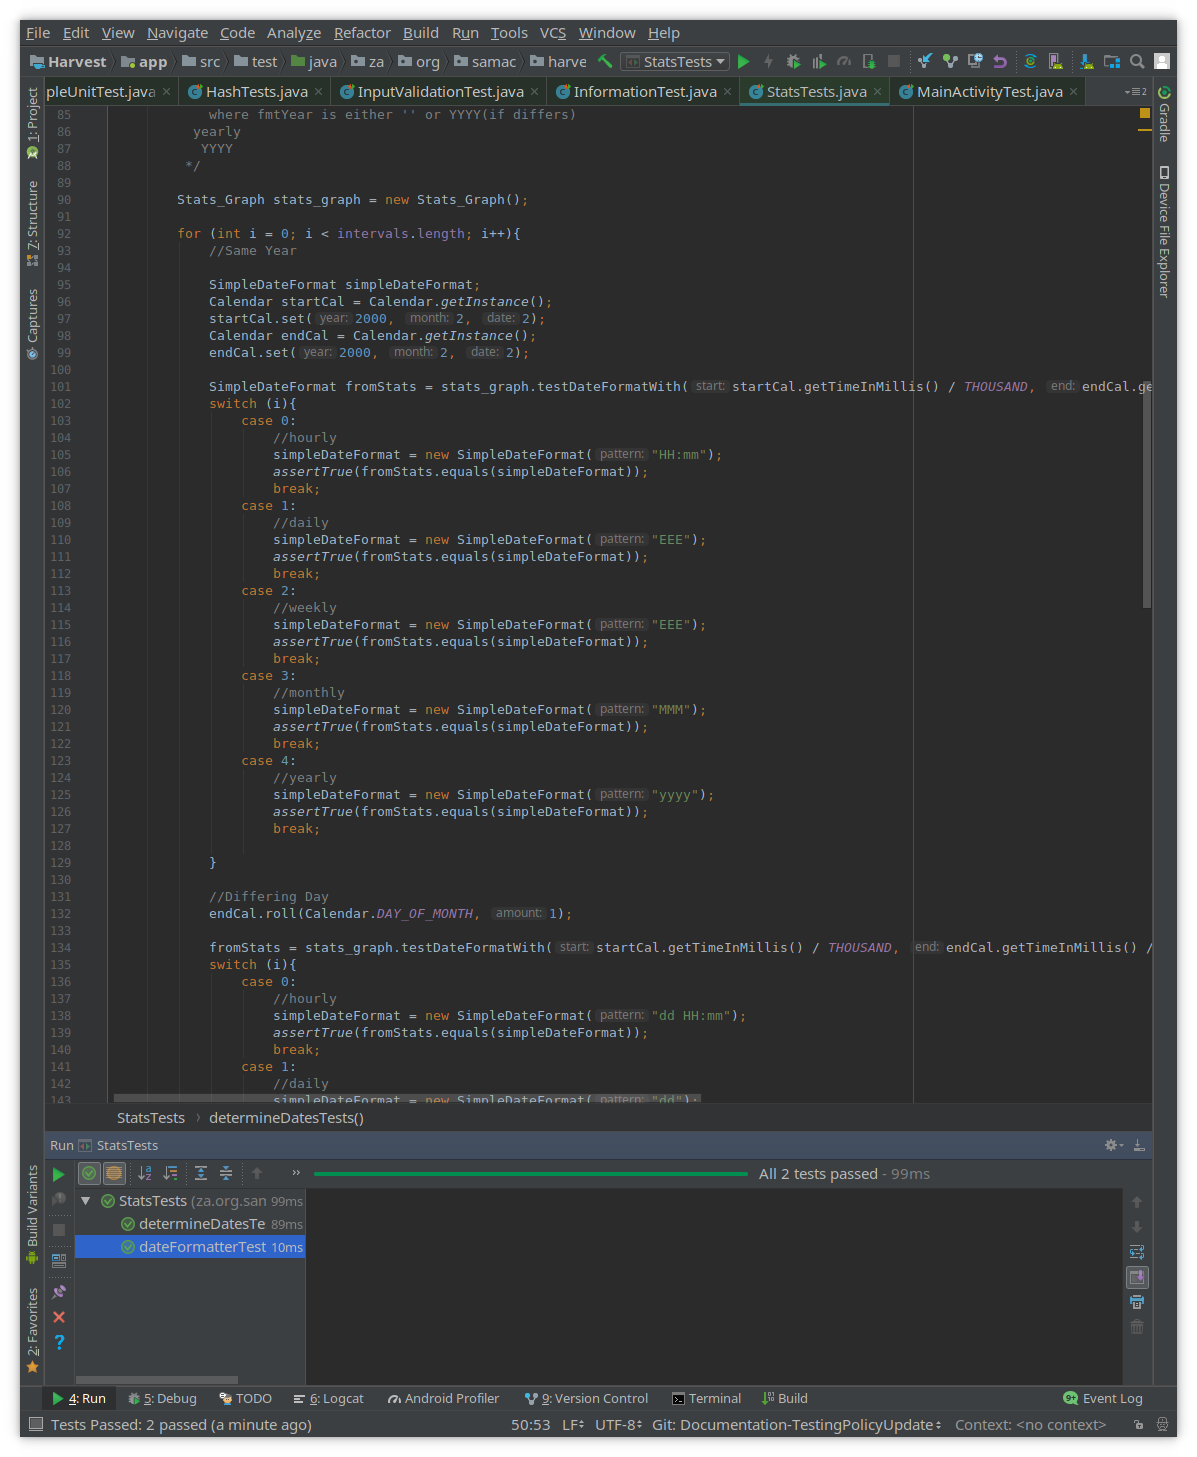
\includegraphics[width=.3\textwidth]{images/stats.png}
            \caption{Unit Test to Verify Functioning of Hash Function}
                        \label{fig:androidsamples}
            \caption{UI Test to Verify Functioning of Information Editing}
            \label{fig:as2}
            \caption{Unit Test to Verify Formatting of Dates}
            \label{fig:as3}

        \end{figure*}
Android test logs can found \href{https://github.com/BinaryNinjaz/COS301-Capstone/tree/master/Source/Android/Harvest/test-logs}{here}. Refer to figures \ref{fig:androidsamples}, \ref{fig:as2}, and \ref{fig:as3} for examples of tests.
\subsection{iOS}
	\begin{figure}
  	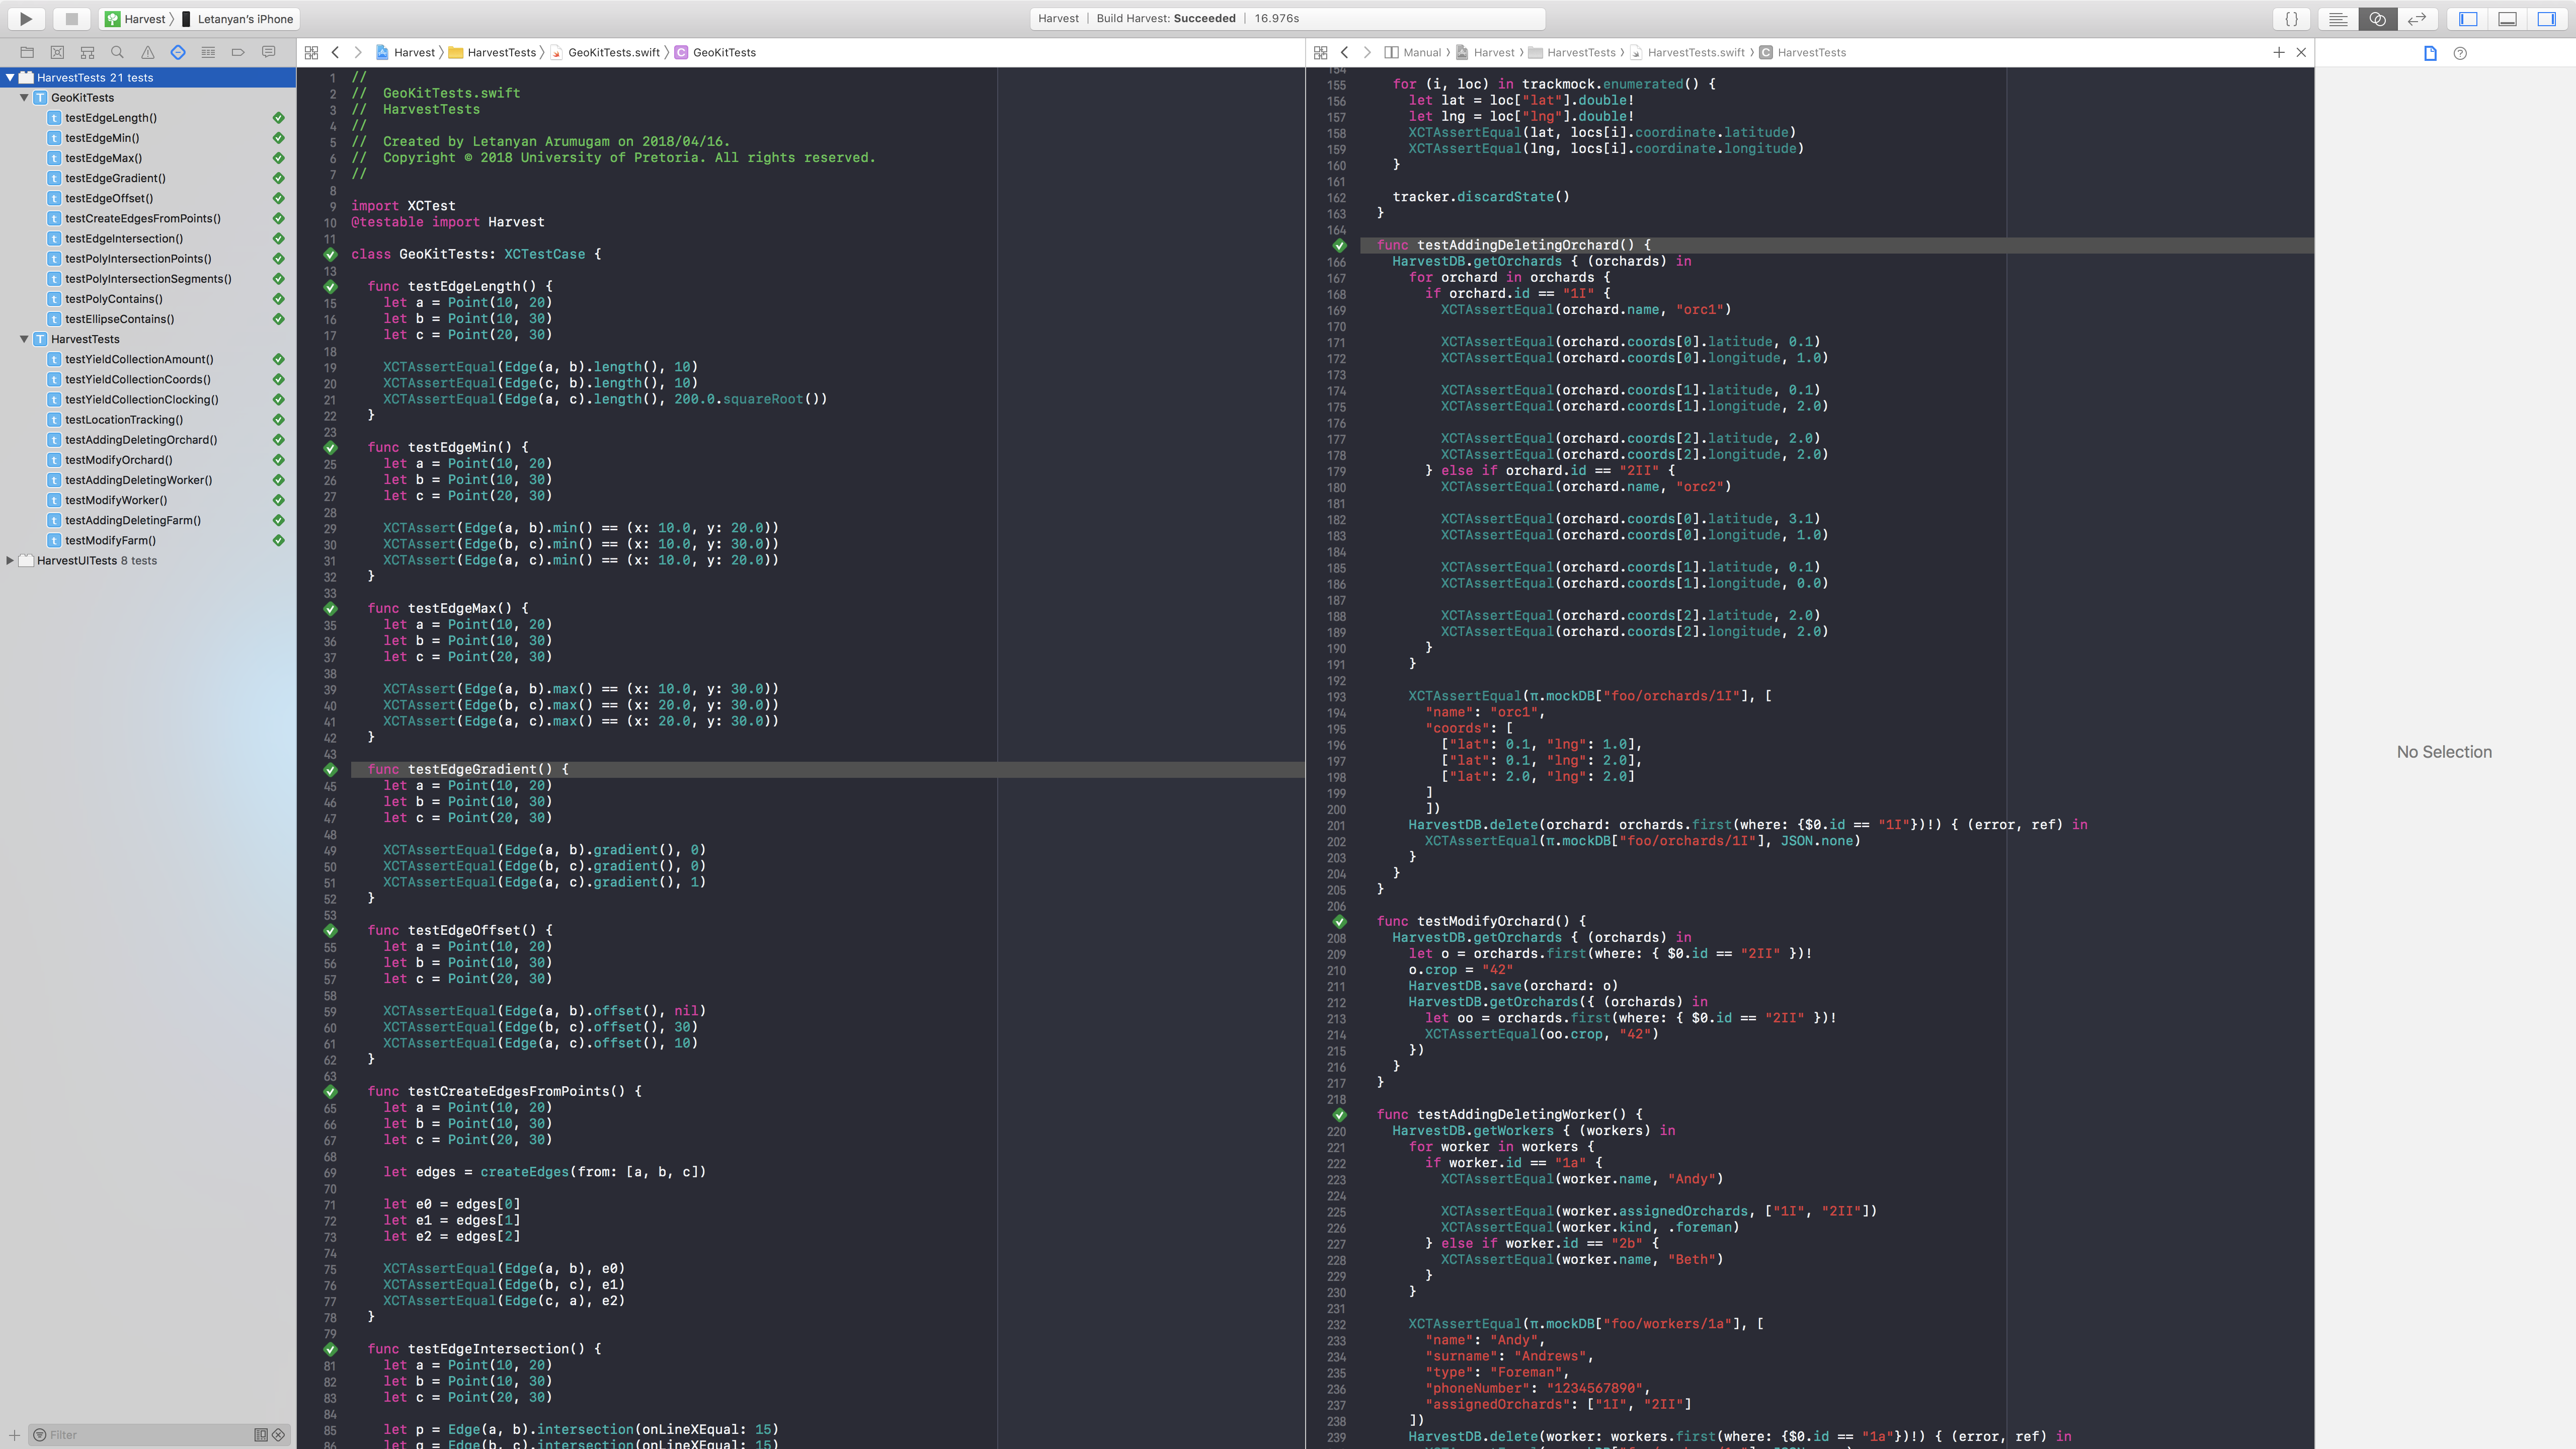
\includegraphics[width=\textwidth]{images/iosexample.png}
	\caption{iOS Xcode Test Example}
	\label{fig:ie}
  \end{figure}
iOS test logs can be found \href{https://github.com/BinaryNinjaz/COS301-Capstone/tree/master/Source/iOS/Harvest/TestResults}{here}.\\
\indent Refer to figure \ref{fig:ie} to see iOS tests.
\subsection{Web}
	\begin{figure}
  	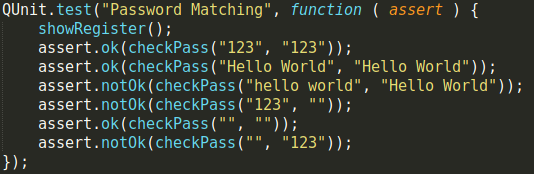
\includegraphics[width=\textwidth]{images/qt.png}
	\caption{QUnit Test to Verify Passwords are Rejected or Approved Appropriately}
	\label{fig:qt}
  \end{figure}
Web test logs can be found \href{https://github.com/BinaryNinjaz/COS301-Capstone/tree/master/Source/Web/test-logs}{here}.\\
\indent Refer to figure \ref{fig:qt} for an example of a QUnit test.
  
\end{document}
